%*******************************************************************************
%*********************************** First Chapter *****************************
%*******************************************************************************

\chapter{Introduction}  %Title of the First Chapter

\ifpdf
    \graphicspath{{Chapter1/Figs/Raster/}{Chapter1/Figs/PDF/}{Chapter1/Figs/}}
\else
    \graphicspath{{Chapter1/Figs/Vector/}{Chapter1/Figs/}}
\fi

Almost any application domain of information systems has some data that is being generated. In many cases this data contains valuable knowledge which can be learned or extracted from it. So what kind of knowledge is this an how is it valuable? This obviously depends on the application domain. For example correlations like \textit{"95\% of all patients that were treated with medication B complained about severe headaches in the following days"} or \textit{"four out of five users who liked the movie Dr. Strange also liked Captain America: Civil War"} clearly represent valuable knowledge for their respective domains. Of course, the time of manual data processing has long since passed as automated, algorithmic solutions were discovered. The field of research that deals with these approaches and algorithms has many different names and subareas with sometimes subtle differences, ranging from data mining, data analytics and data analysis to machine learning or business intelligence to only name a few. \\
The underlying data, which is processed to reveal knowledge can of course take many forms. One very general category of this data are data streams. Data streams are not limited to the recent rise in popularity of video and audio streams. On the contrary the application domains that produce data in the form of streams are very diverse. They include for example constantly running business applications that log business activities and events, sensor networks that report usage data or devices that take measurements of physical quantities (such as temperature, pressure, humidity, etc...) at certain points of time. \\
The fact that streams generate a constant stream of data and thus lead to a constantly growing amount of data is a significant difference to classic applications of data mining in which there is a static (training) database. Despite that significant difference, many fields of interest in the context of static databases are also of interest for data streams. Approaches and algorithms that solve problems for static databases, while by no means fully researched, are rather well known and evaluated. Applying these methods to data streams can present challenges and may demand many modifications due to the large and possibly infinite amounts of data produced by streams. Naturally, data mining methods for stream data must be especially fast, scalable and memory efficient. \newline
Apart from the additional, algorithmic constraints on memory and computation time, data streams also present conceptual challenges. In contrast to static databases streams may evolve over time, which can make it very difficult for algorithms to assess which past data of the stream should be considered when analyzing the currently incoming data. Recognizing these so called concept drifts is one challenge among many when processing or mining data streams. \newline
A suitable way to look at most data streaming scenarios is that of event streams. An event can be basically anything that happens in the real world, represented as an element of a data stream. Examples of this could be a rise in temperature that is reported by a sensor or an increase in the value of a stock, that is being traded at a stock market. In the context of event processing, events are commonly referred to as basic or simple events. \newline
A more advanced form of events are complex events. Complex events are structures that consist of multiple basic events with different relationships between each other. Discovering interesting complex event patterns can be tough, especially since there may be a lot of potential candidates. The discovery of complex events is related to the research area of pattern mining, since complex events are essentially large patterns, that are mined from basic events. Traditionally, pattern mining is an area of data mining that is often employed to extract knowledge or interesting correlations. Discovering interesting complex events in an event stream is called complex event pattern mining. However, in addition to the underlying event stream, this thesis aims to also use semantic knowledge to improve or extend the results of the mining process. Semantic knowledge is essentially additional information about the events present in the stream. Simple domain knowledge like \textit{"Sensor A was built by company XY"} or \textit{"Company A belongs to the IT-Sector"} can have big implications for the interestingness of patterns. Considering additional domain knowledge in the mining process what we refer to as semantic complex event pattern mining. \\
Since the term of complex events is very broad this thesis will focus on the subtopic of episode patterns. Episodes are a specific kind of complex events and are formally defined in chapter \ref{chapter_related}. For now it is sufficient to know that episodes are essentially complex events in which single events or entire episodes can be combined using two operators: the conjunction and the sequence operator. Figure \ref{fig_simpleEpisodeExample} visualizes a simple episode pattern and example occurrences in a data stream.

\begin{figure}[h]
	\centering
  	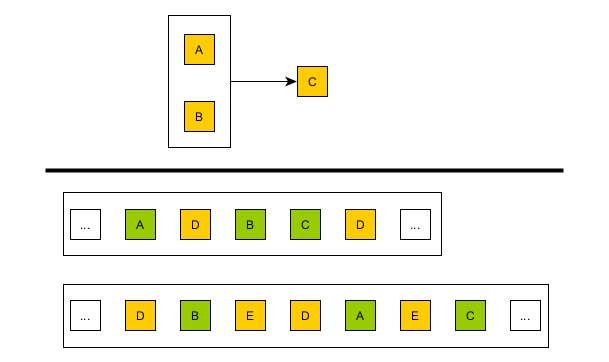
\includegraphics[width=0.5\textwidth]{exampleEpisode.jpg}
	\caption{The top half visualizes an example episode pattern, which consist of a conjunction (A and B must both occur, but the order does not matter) and a sequence (C must occur after A and B). The bottom half shows two windows of an example stream, in which occurrences of the episode are shown in green.}
	\label{fig_simpleEpisodeExample}
\end{figure}

Episodes are sequential patterns that have previously been mined from very long sequences, which makes them an appropriate mining target in event streams, since streams and sequences share the sequential nature. The only difference is that streams grow over time, whereas sequences have a fixed size.\\
The main question now is: why should we be interested in complex events or episodes? What benefit does the discovery or recognition of such structures in a data stream have? While there are indeed many uses for the discovery of complex events this thesis will focus on one specific application: Prediction. The prediction of certain events in an ongoing event stream has many obvious use cases such as building early warning systems for hazardous events like power outages in power grids, failures in sensor networks or even natural disasters, such as earthquakes. Prediction in itself is of course a widely researched topic, but building predictive models based on complex event mining results has, to the best of the authors knowledge, not been explored yet.
The idea of how to combine these two research area is rather simple. We aim to mine complex events from an event stream with the specific purpose of predicting future occurrences of a specific event type. As mentioned before, when mining complex events we also want to consider semantic knowledge in addition to the data present in the stream. \newline
Figure \ref{fig_approach} summarizes the goal of this thesis graphically. The underlying event stream is mined for complex events by a mining algorithm that will consider the information given in the stream as well as the semantic knowledge. The resulting complex events are then used as input for a model building algorithm, which will produce a predictive model. Afterwards this model can be used to predict occurrences of certain events in the original (still ongoing) event stream.
\begin{figure}[h]
	\centering
  	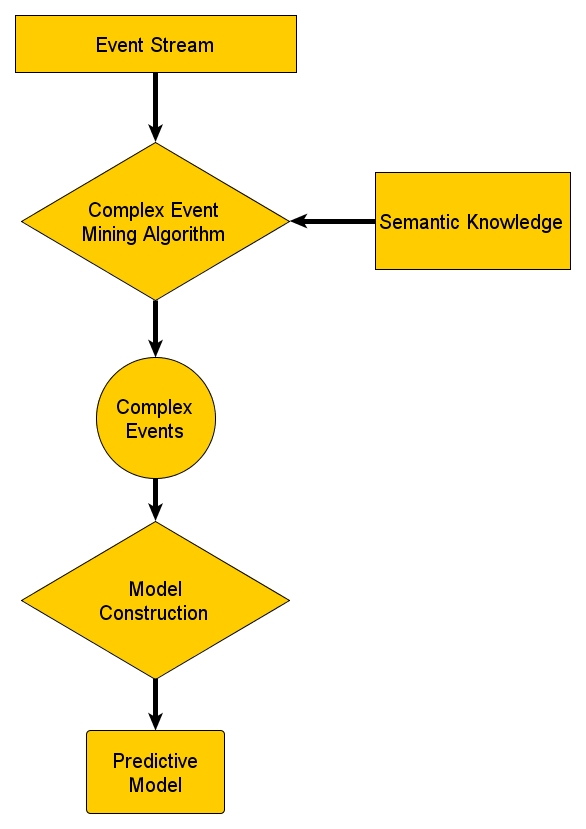
\includegraphics[width=0.5\textwidth]{approach.jpg}
	\caption{General Structure of the approach suggested by this thesis.}
	\label{fig_approach}
\end{figure}

The domain that will be used in the evaluation of this thesis is stock market prediction. Both predicting the overall direction of the stock market and predicting whether individual stocks will rise or fall are a difficult problems that have the obvious application of making profitable investments. \newline
The rest of the thesis is outlined as follows: Chapter \ref{chapter_related} introduces the basic terminology and reviews the related work, Chapter \ref{chapter_background} follows up with formal definitions and a more detailed introduction to episode mining. Chapter \ref{chapter_solutions} presents the suggested algorithms to mine predictive models for event streams using episodes and analyzes their complexities. Subsequently chapter \ref{chapter_evaluation} presents an extensive evaluation using real stock market data. Finally chapter \ref{chapter_conclusion} concludes the paper and mentions possible future work.


%TODO use this somewhere
%In contrast to other regression and forecasting methods, such as artificial neural networks, predictive episodes have the advantage that once they are discovered they can make ad-hoc predictions in a fast moving data-stream, whereas neural networks usually forecast the closing values of stock markets of the next day based on the values of previous days. This gives predictive episodes a niche: fast moving (real-time) data-streams that need quick predictions of future events. \newline

%TODO move this
%\section{Problem Definition and Exact Research Question}
%Even though many terms have not yet been precisely defined (which will be done in chapter \ref{chapter_related} ) this section presents a loose, intuitive definition of the problem to be tackled by this thesis. Given a stream of basic events and a special event type $P$ one is interested to predict occurrences of that special event type $P$ in the stream, so that actions can be taken before $P$ actually occurs. For this purpose we are interested to discover episodes in the stream of which occurrences are temporally correlated to the occurrence of $P$. A window of an example stream is visualized in figure \ref{fig_predictiveEpisodeExample}. In this simple example the episode $A$ followed by $E$ always occurs before $P$.
%
%\begin{figure}[h]
%	\centering
%  	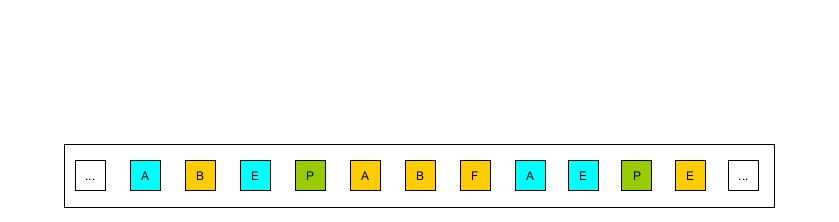
\includegraphics[width=0.6\textwidth]{examplePrediction.jpg}
%	\caption{The figure visualizes an event stream in which events of type $P$ are to be predicted. The occurrences of the episode $A$ followed by $E$ is colored in teal, whereas events of types $P$ are colored in green and all other events are yellow}
%	\label{fig_predictiveEpisodeExample}
%\end{figure}
%
%Note that it is very important to the mining process how much time is allowed to pass between the occurrence of the mined episode and the event that is to predict. If this time span is too small a mining algorithm might not find reliable correlations. If the timespan is too large a mining algorithm might be overwhelmed by the number of candidates that need to be considered, since the more time may pass the larger are the sequences before each event $P$ that must be considered. %TODO maybe move the last sentences to method? 
%\newline
%To solve the problem outlined above a semantic mining algorithm will be suggested in this thesis. Since the underlying data structure to be analyzed are data streams, the algorithm must have the following properties:
%\begin{itemize}
%	\item The algorithm must be able to adapt to a changing context (as the stream progresses, the underlying correlation may change completely)
%	\item The recognition of episodes must be quick, since streams, especially in the domain of stock markets, can have a high velocity. This makes it important to be able to quickly predict events. If the prediction takes too long, the event which we want to predict may have already occurred before the algorithm outputs its prediction, thus robbing the user of the opportunity to take action.
%	\item The Algorithm must not require to store the entire stream of events seen so far, since that is not feasible for most streams.
%\end{itemize}
%
%The algorithm will be evaluated on real-life data-sets from the domain of stock market prediction, in which the developed algorithm will be empirically compared to other approaches in terms of accuracy measures and execution time. In summary the research question in particular is:\newline \newline
%\textbf{How can event streams be mined for episodes that help predict certain event types and how can domain knowledge be used to improve the results of the mining algorithm?}